Projects overview displays all user's projects and allows users to create a new project or import an existing project (Figure~\ref{fig:projects_overview}).
The project list shows the title and description of each project in a separate line.
After clicking on a project its line expands and processes are displayed in a form of chips.
Each chip shows the process icon and title.
At the bottom of the expanded line there are buttons for managing the process.
Delete button will permanently remove the project.
Open button will navigate the user to \hyperref[sec:project-detail]{Project Detail} view.

\begin{figure}[h!]
  \centering
  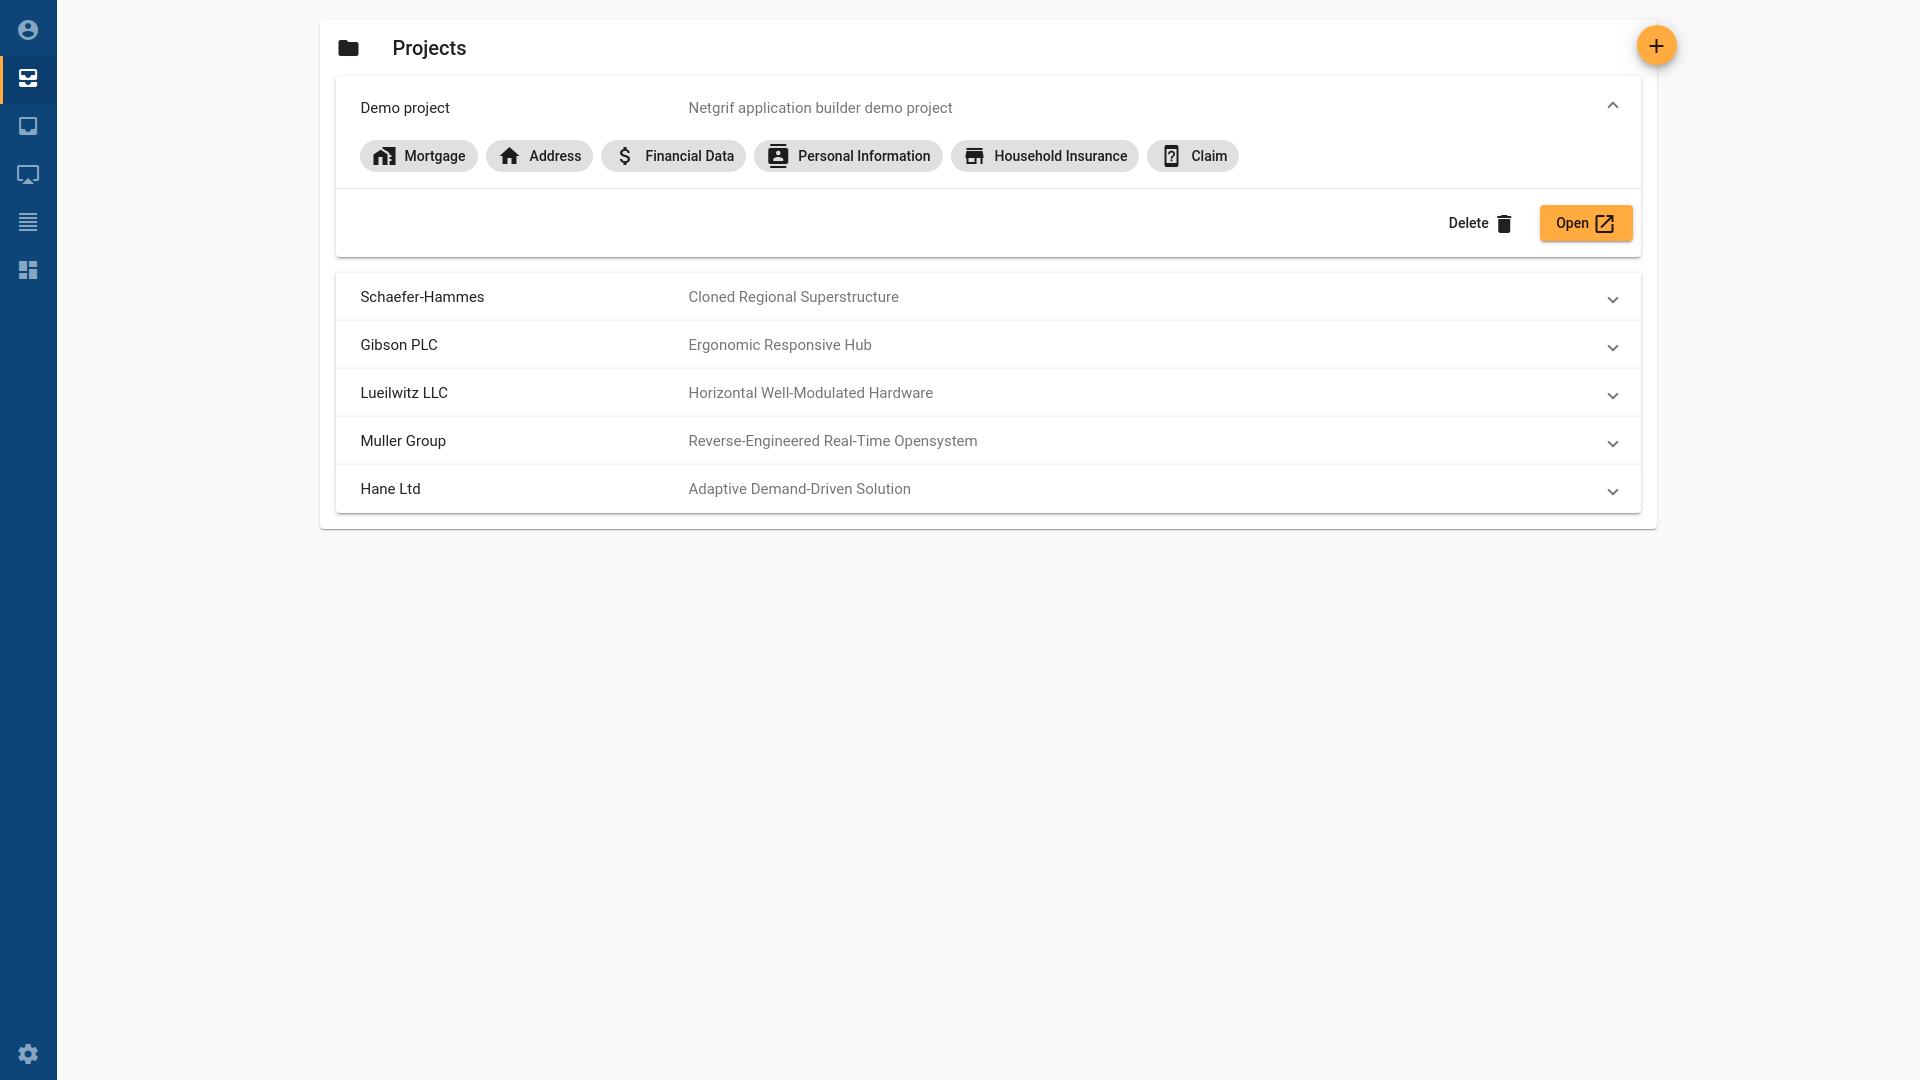
\includegraphics[width=0.9\textwidth]{images/projects_view.png}
  \caption{Projects overview}
  \label{fig:projects_overview}
\end{figure}

Clicking on the fast action button on the right side will show two options for creating a new project.
The first option is to create a new empty project.
Importing an existing project is the other option, which will open a file dialog where you can select an existing project on your device.

Projects are currently not saved to any server and leaving the \builder~will result in the loss of all projects.
